% ==========================
% ŠABLONA XETEX ČLÁNEK
% ==========================


\documentclass[a4paper,12pt]{article}

% ==========================
%	Balíčky
% ==========================
%\usepackage[czech]{babel}		% nastavení češtiny (dělení slov, odstavce, nadpisy, datumy...)
%\usepackage[utf8x]{inputenc}		% nastavení vstupního kódování na UTF8
%\usepackage[T1]{fontenc}		% kodování fontu pro výsledný dokument

\usepackage{listings}
\lstset{language=C++, numbers=left, backgroundcolor=\color{Azure}}

% podpora jazyků
\usepackage{polyglossia}

% pro použití obrázků
%\usepackage[pdftex]{graphicx}			

% pro podporu výpisů programu
\usepackage{listings}

\usepackage{hyperref}

% pro definování vlastních barev - lepší než color
\usepackage[svgnames]{xcolor}						

% pro více obrázků u sebe s jednou popiskou
\usepackage{subcaption}		

% matematika vlepší a abstraktnější verzi
\usepackage{amsmath}

% ==========================
%	Nastavení
% ==========================			

\graphicspath{ {./obrazky/} }

% počeštění názvu výpisu kódů
\renewcommand{\lstlistingname}{Kód}



\definecolor{bluekeywords}{rgb}{0.13,0.13,1}
\definecolor{greencomments}{rgb}{0,0.5,0}
\definecolor{redstrings}{rgb}{0.9,0,0}


\lstdefinestyle{sharpc}{
	language=[Sharp]C, 
	tabsize=4,
	keywordstyle=\color{blue}}

\lstset{style=sharpc}



% vycentrování obsahu všech floatů
\makeatletter
\g@addto@macro\@floatboxreset\centering
\makeatother

% vlastní dělení slov
\hyphenation{vy-ge-ne-ro-va-ných}


% ==============================
%	Začátek dokumentu
% ==============================
\begin{document}

% ==============================
%	Titulní strana
% ==============================
\begin{titlepage}

\sffamily	% odtud se píše bezpatkovým písmem

	\begin{center}
		\begin{Large}
		
		Západočeská univerzita v~Plzni

		\vspace*{0.2cm}
		
		Fakulta aplikovaných věd

		\vspace*{0.2cm}
		
		Katedra informatiky a výpočetní techniky
		
		\vspace*{5mm}

		% vložení loga ZČU	
		
\includegraphics[width=0.25\textwidth]{obrazky/logo_zcu}	
		
		\vspace*{2cm}
		
		% Název předmětu
		{\Huge\bfseries Semestrální práce z~předmětu Operační systémy}

		\vspace*{1cm}
		
%		% Název úlohy
		{\bfseries SMP}
		\end{Large}
	\end{center}
	
	% vyplní mezerami do konce stránky
	\vfill

	% vloží čáru o tloušťce 0,4 pt (tloušťka kartonu)
	\hrule
	
	\vspace*{0.2cm}	
	
	% neodsazovat první řádku kontaktu
	\noindent
	Zdeněk Janeček \\ 
	janecekz@students.zcu.cz \\
	A14N0112P \\
	Plzeň, \number\day. \number\month. \number\year

	\vspace*{0.2cm}	
	
	\noindent
	David Fiedler \\ 
	david.fido.fiedler@gmail.com \\
	A14N0111P \\
	Plzeň, \number\day. \number\month. \number\year
	
	\vspace*{0.2cm}	
	
	\noindent
	Tomáš Cigler \\ 
	tcigler@students.zcu.cz \\
	A14N0110P \\
	Plzeň, \number\day. \number\month. \number\year

\rmfamily	% odtud se opět píše patkovým písmem

\end{titlepage}


\section{Zadání}

Cílem semestrální práce je vytvořit simulátor 4 jádrového SMP, pro který se vytvoří plánovač a implementace semaforů.
Semafory budou implementovány tzv. spinlockem a pouze tyto mohou být následně použity k~synchornizaci procesů.

Pro každý procesor bude vytvořeno vlákno simulující obsluhu přerušení hodin, ve kterém se bude měnit kontext pracovního vlákna. Pracovní vlákno bude simulovat fyzický procesor. Na výběr je buď vytvořit idle procesy v~počtu procesorů, aby bylo co plánovat, když bude málo runnable threadů, anebo naimplementovat halt stav procesoru. Nesmí se ovšem zastavit všechny procesory - alespoň jeden musí zůstat vzhůru - tj. minimálně jeden idle proces musí být.

V~systému bude spuštěno osm úloh producent - konzument. Producent bude generovat náhodná čísla v~plovoucí čárce s~normálním rozdělením dle zadaných parametrů. Konzument z~nich bude průběžně počítat parametry normálního rozdělení.
Průběžně se bude ukazovat konvergence vypočítaných parametrů k~zadaným, včetně počtu zpracovaných hodnot.

Bude vytvořeno rozhraní, kterým bude možné pozastavovat jednotlivé thready, a celkově program ovládat. Ukazujte využití jednotlivých procesorů.

Tato aplikace bude z~povahy zadání cílena jen na architekturu \emph{Intel x86}.

\section{Návrh}
Prvním krokem je běžící procesor. Každé jádro je jedno běžící vlákno, na němž se provádí instrukce = úlohy. Plánovač je také úloha, proto by měl být pomocí přerušení plánován na procesor. Jelikož máme použít metodu Round Robin, stačilo pouze přerušení po časovém limitu. Pro udržení procesoru v~běhu jsme zvolili jeden idle task.

Plánem bylo izolovat úlohy od procesoru i plánovače - na instrukcích dané úlohy nezáleží a musí běžet a plánovat se plně nezávisle. Úloha producenta a konzumenta ale přesto musí být spolu v~kontaktu. 
Z~toho důvodu jsme se vydali směrem společné procedury pro vytvoření úloh. Prvních osm běžících úloh bude vytvořeno ihned po startu celého systému a naplánováno pro běh.

Konzole bude monitorovat stav procesoru, resp. jader a následně poskytne možnost ovládat plánovač.

\section{Implementace}

\subsection{Virtuální SMP}
Spouštění procesoru probíhá obdobně jako u~reálného procesoru. Vstupem je procedura
\verb+hardware_start+. Nejdříve se inicializuje
systém obsluh přerušení. Každé přerušení je mapováno na samostatný Handler
hostitelského systému. Použil jsem úplně základní Event. Ten je v~počátečním stavu
nesignalizovaný. Každé přerušení lze také zamaskovat a má svojí obslužnou rutinu.

V~naší aplikaci jsou k~dispozici následují přerušení.

\begin{description}
\item{INT\_SCHEDULER} Přepnutí plánovače. Běží typicky na prvním procesoru. Ostatní
jádra mají toto přerušení zamaskované.
\item{INT\_RESCHEDULE} Přepnutí úlohy na procesoru. Toto přerušení očekává adresu
zásobníku v~příslušné zprávě.
\item{INT\_CORE\_TERM} Ukončení jádra.
\item{INT\_CORE\_RESUME} Opětovné spuštění. Používá plánovač.
\item{INT\_CORE\_SUSPEND} Pozastavení jádra.
\end{description}

Prvním vzniklým vláknem je vlákno hardwarového přerušení, které slouží k~signalizaci
plánovače. Stará se také o~životní cyklus celé simulace SMP. Toto vlákno simuluje
fyzické zapojení a tedy běží s~nejvyšší prioritou.

Každé jádro má svoje vlákno obsluhy přerušení. To odpovídá hodinám, kde nebyly třeba
ve své původní podobě, protože instrukce obslužného jádra běží nezávisle na hodinách
jako nativní kód. Při inicializaci vlákna obsluhy přerušení vznikne také fyzické jádro.

Dále se inicializuje plánovač. To je první úloha, která se spustí na prvním procesoru.
Plánovač si vytvoří základní kontext, ze kterého pak vznikají další odvozené. Mimo inicializace
paměti vytvoří první přerušení plánovače. Plánovač zavede první jádro a začně provádět
svůj kód. Více o~plánovači v~další části.

Vypnutí procesoru zajistí procedura \verb+power_button+. Ve skutečnosti vznik\-ne event,
na který obslužné vlákno hardwarového přerušení zareaguje a rozešle sadu přerušení pro
ukončení všech jader. Po ukončení procesoru, provede se také ukončení všech otevřených
handlerů přerušení.

\subsection{Obsluha přerušení}
V~předchozí sekci jsem se již zmínil o~technickém provedení přerušení a to systémové
události, na která čekám pomocí \verb+WaitForMultipleObjects+. Některá přerušení mají
obsluhu, která běží na cílovém procesoru, ale některá slouží k~ovládání jádra.
Z~těch co běží na jádře jsme si vystačili s~obsluhou plánovače a přeplánování.

Přerušení plánovače \verb+INT_SCHEDULER+ nejdříve získá vnitřní zámek plánovače aby
nedocházelo k~souběhu s~některým systémovým voláním. Pak pozastaví všechna jádra a uloží jejich kontext. Jádru je tím předložena instrukce obsluhy, která použije svůj zásobník plánovače.
Plánovač pak vrátí přes registr EAX adresu následujícího zásobníku. Ten je načten běžnou cestou.
Návrat do přerušené úlohy je přes instrukci RET. Na prvním procesoru vždy něco běží.

Díky tomu je možné přeskládat úlohy s~jejich aktuálním stavem. Kontext na zásobníku
obsahuje návratovou adresu tj. následující instrukce úlohy, stavové vlajky a pak všechny
registry v~pořadí jak je vyžaduje instrukce \texttt{popad}.

Přerušení přeplánování \verb+INT_RESCHEDULE+ pozastaví cílové jádro a počká na zámek
plánovače aby mohlo uložit celý kontext aktuálně běžícího vlákna. Z~matice zpáv si přečte
cílový ESP, který vloží do kontextu jádra. Stejně tak jako v~předchozím případě. Vloží
do EIP adresu obsluhy přeplánování. Cílové jádro je probuzeno.

Obsluha přerušení je napsána v~Assembleru, abych nepoškodil kontext přerušené úlohy. Využívám tak
instrukce \texttt{popad} pro načtení obecných registrů a  \texttt{popfd} pro načtení vlajek.

\subsection{Plánovač}
V~těle plánovače dojde nejdříve k~ověření, zda nebylo pozastaveno nějaké jádro. To je
způsobeno zavoláním voláním plánovače \verb+sched_request_resume+ a \verb+sched_request_pause+.
Jakmile něco běží na pozastaveném procesoru, musí se to pozastavit a uložit kontext.
Tato úloha pak putuje na konec fronty úloh.

Dále se mažou všechny úlohy které ukončily své tělo. Struktura TCB obsahuje destruktor,
takže jsou v~tu chvíly uvolněny veškeré alokované pro\-středky.

Ještě před spuštěním samotného plánovaní jsou načteny požadavky na nové úlohy. To zahrnuje
vytvoření nového Task Control Block (TCB). O~inicializaci dat se stará funkce
\verb+sched_create_task+. Zásobník musí být souvislý a zarovnaný. Vložíme do něj postupně:

\begin{itemize}
\item argument úlohy
\item návratová adresa do endtask callbacku
\item vstupní adresa úlohy
\item vlajky
\item obecné registry
\end{itemize}

Na hodnotách registrů nezáleží. Vkládám tam nějaké hodnoty abych poznal že
se vše načítá správně. Dále je nastaven Task ID (TID), časové kvantum, stav Runnable,
typ úlohy a také předávaná struktura, kvůli dealokaci paměti.

Činnost plánovače je pro každé jádro stejná:

\begin{itemize}
\item ověříme zda je jádro povolené
\item podíváme se do tabulky spuštěných procesů na proces co na jádru běží. Jestliže tam nic neběží
pokračuje v~další části.
\begin{itemize}
\item ubereme mu časové kvantum TIME\_QUANTUM\_DECREASE
\item pokud už běžící proces vyčerpal čas TIME\_QUANTUM, zařadí se do fronty procesů.
IDLE task v~tu chvíli končí. Pokud kvantum nevypršelo je navrácen zpět mezi naplánované úlohy a pokračuje
dalším jádrem.
\end{itemize}
\item podle fronty úloh
\begin{itemize}
\item Je-li prázdná a jsme na prvním procesoru, je spuštěn IDLE task. Jsme-li na jiném jádře. Je to
jádro pozastaveno.
\item máme-li čekající úlohu ve frontě, je vybrána jako následující
\end{itemize}
\item pokud je vybraná úloha ta stejná která tam byla před přeplánováním, je tato změna ignorována
\item Nakonec proběhne samotné přerušení cílových jader a odeslání cílového ESP. První jádro je
přeplánováno při návratu z~plánovače.
\end{itemize}

\subsection{Životní cyklus úlohy}
Nyní popíšeme životní cyklus aplikace od jejího vzniku, stavy běhu a nakonec její
ukončení. Naše schéma je na obrázku \ref{fig:state_diagram}. Z~běžného schématu
vypadl stav blokovaný, protože používáme aktivní čekání a není k~dispozici
přerušení na úrovni instrukcí, ale pouze signalizace.

\begin{figure}
\centering
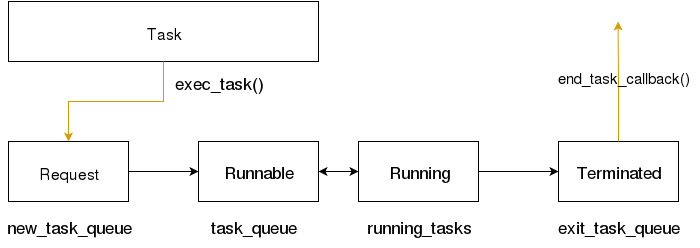
\includegraphics[width=\textwidth]{obrazky/state_diagram.png}
\caption{Stavový diagram úloh}
\label{fig:state_diagram}
\end{figure}

Každá úloha může spouštět jiné úlohy, a to pomocí volání \verb+exec_task()+. Prvním
parametrem funkce je typ úlohy a další je ukazatel na strukturu parametrů. Záleží na typu úlohy a
může být i NULL. Tento ukazatel může být mezi úlohami samozřejmě sdílen. Proto je také
typován jako \verb+shared_ptr+ aby byl po skončení "uklizen". Není hlídána cyklická
reference.

Jakmile se naplánuje plánovač projde frontu nových úloh, vytvoří jejich TCB a zařadí
do fronty čekajících úloh v~\verb+task_queue+.
Až se na ni dostane řada, přejde do stavu RUNNING. Plánovač zajistí přepnutí úlohy.

Každá úloha se může nacházet jen v~jedné z~těchto front. Proto je také TCB unikátní pointer.
Jeho prostředky jsou automaticky uvolněny po vymazání z~fronty
\verb+exit_task_queue+. Do té se dostane při návratu z~hlavní procedury v~metodě
\verb+end_task_callback()+. Ta je vložena do zásobníku při vytváření a tedy instrukce
RET do ní skočí.

\subsection{Systémová volání}
Každé systémové volání je definováno v~modulu \verb+sched_calls+. K~dispozici
je již zmíněné \verb+exec_task()+ a také \verb+get_tid()+. Tato volání jsou přímo
mapována na volání plánovače. To je z~důvodu odstínění úloh od plánovače. Tyto
volání jsou přesto volána synchronně a jsou co nejkratší.

Jednotlivé úlohy získávají parametry z předem známých struktur.

\newpage

\begin{lstlisting}
struct task_common_pointers {
	semaphore_t full;
	semaphore_t empty;
	semaphore_t mutex;

	circular_buffer buffer;

	std::atomic<bool> can_run;
	double mean;
	double deviation;

	std::atomic<double> mean_diff;
	std::atomic<double> deviation_diff;
	std::atomic<int> processed;
};
\end{lstlisting}

Tato struktura slouží pro nastavení úloh PRODUCENT a CONSUMENT. Pro spuštění
RUNNER je třeba naplnit:

\begin{lstlisting}
struct task_run_parameters {
	double mean;
	double deviation;
};
\end{lstlisting}

\subsection{Synchronizační primitiva}
Pro potřeby jak úloh, tak vnitřních struktur bylo potřeba implementovat vlastní
semafor. Knihovní funkce totiž nefungují. Z~pohledu systému máme pouze 4 vlákna
procesoru, ale ve skutečnosti synchronizujeme mezi neexistujícími úlohami.

Definovali jsme tedy strukturu \texttt{semaphore\_t}, která uchovává aktuální hodnotu
semaforu. Tělo takového zámku je v~následujícím výpisu. Nechávám zde pro snažší
pochopení Assemblerové implementace.

\begin{lstlisting}
int semaphore_P(semaphore_t &s, int value)
{
	int expected;
	int old;

	do {
		do {
			old = s._value;
			expected = old - value;
		} while (expected < 0);
	} while (!s._value.compare_exchange_weak(
		old, expected,
		std::memory_order_release,
		std::memory_order_relaxed));

	return expected;
}
\end{lstlisting}

Kód semaforu byl použit následující (\texttt{synchro.cpp}):

\lstset{language=[x86masm]{Assembler}}

\begin{lstlisting}
spin:
	mov edx, s
	mov edx, [edx]s._value
	mov ebx, edx
	sub ebx, value
	js spin

	mov eax, edx
	; eax - old, [ecx]s - actual, ebx - expected
	mov ecx, s
	lock cmpxchg[ecx]s._value, ebx
	jnz spin
	mov result, ebx
\end{lstlisting}

\lstset{language=C++}

Vzhledem k~tomu že jsem cílil na x86, mohl jsem použít inline assembly
a obalit standardní funkcí.

Uvolnění hodnoty semaforu je jednoduché:

\begin{lstlisting}
void semaphore_V(semaphore_t &s, int value)
{
	s._value += value;
}
\end{lstlisting}

\subsection{Konzole}

\begin{figure}
\centering
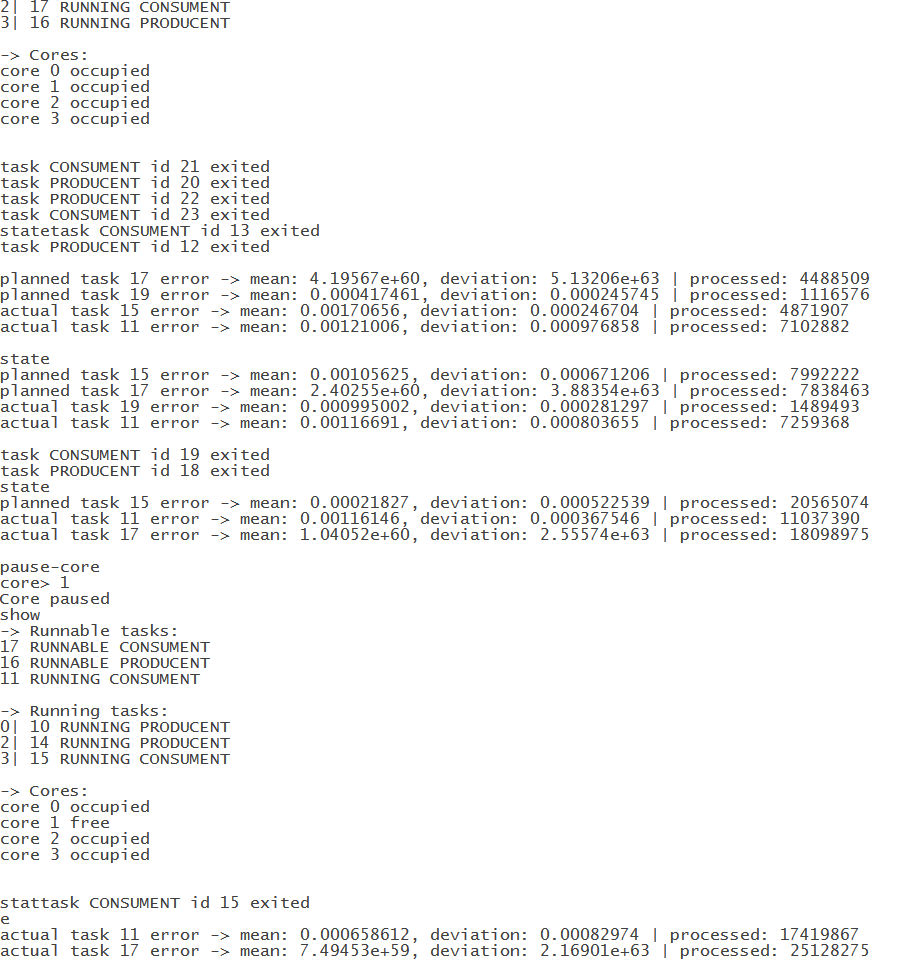
\includegraphics[width=\textwidth]{obrazky/screen.png}
\caption{Screenshot obrazovky}
\label{fig:screen}
\end{figure}

Konzole slouží k~ovládání a monitorování běhu systému. Uživatel zadá příkaz a podle něj se vyvolá obsluha.
Příklad je na obrázku \ref{fig:screen}.

\begin{itemize}
\item exit: vypne program
\item start: spustí úlohu
\item help: ukáže nápovědu
\item show: ukáže informace o~běžících procesech,čekajících procesech a obsazenosti CPU
\item state: zobrazí aktuální chybu výpočtu v~úlohách. Tato funkce je volána pravidelně.
\item pause-core: pozastaví jádro procesoru
\item resume-core: znovu spustí jádro procesoru
\end{itemize}

\section{Referenční úlohy}
Pro otestování funkčnosti celého systému byl podle zadání vytvořen vzor úlohy producent - konzument tak, že producent vytváří
náhodná čísla z~normálního (Gaussovského) rozdělení. Konzument tato čísla zpracovává a počítá inkrementálně zpětně parametry rozdělení, což je střední hodnota a rozptyl.

Aby mohly úlohy spolupracovat, je třeba nastavit jim společné parametry. Mezi ně patří cyklický buffer, přes který
předává producent konzumentovi vygenerovaná čísla. Přístup do bufferu a ochrana před přetečením je řízen dvěma semafory.
Jeden semafor slouží pro udržení počtu prázdných, druhý k~počtu obsazených míst bufferu. Třetí semafor je binární a zajišťuje synchronizaci při přístupu do kritické sekce, kde se vybírá číslo přítomné v~bufferu.

Tyto semafory jsou inicializovány ještě před spuštěním samotných úloh. Jak již bylo řečeno, spuštění obou těchto úloh
zajišťuje pouze jedna funkce, a to \verb+task_main_runner+. Do té se předají parametry rozdělení, uvnitř se inicializují všechny společné parametry a vytvoří se obě úlohy. Tento přístup je výhodný také z~důvodu možnosti vytvoření této dvojice úloh z~uživatelské konzole.

Reálné parametry rozdělení musí znát i konzument, aby bylo jasné, kdy má úloha skončit. Inkrementálním způsobem se parametry počítají tak dlouho, dokud přesnost výpočtu podléhá větší chybě, než je povolená tolerance. Vzhledem k~zaokrouhlovacím chybám, nepřesnosti číselných typů a diskrétním hodnotám generování není konvergence příliš rychlá. Nicméně při toleranci řádově v~setinách se původním parametrům přiblíží výpočet již po několika tisísích vzorcích. Po dosažení přesnosti signalizuje konzument producentovi ukončení.


\section{Závěr}
Při vypracování této úlohy jsme narazili na mnoho problémů, které je třeba
řešit a prozkoumali jsme základní úlohu operačního systému a to sdílení réalného času.
Využili jsme jak vysokoúrovňového C++, tak Assembleru. Zaměřili jsme se na starší
archetekturu Intel x86, protože nevyužívá velké množství registrů než 64 bitová
následovník. Z~tohoto důvodu nejspíše zmizeli zásadní instrukce \texttt{popad} a \texttt{popfd},
které přečtou zásobník a přepíší registry. Na reálném procesoru je obsluha přerušení řešena
hardwarově a proto je možné obsluhovat s~takovou rychlostí.

Bylo třeba dát si pozor co skutečně překladač vytvoří. Narazil jsem na problém, když jsem
měl nastavený malý zásobník a překladač tiše předpokládal větší. Pak nastalo k~překryvu
adresního prostoru zásobníku a datového segmentu. Překladač totiž zahrnuje do kódu různé
čištění paměti pomocí instrukce \verb+rep stos+. Všechny takové chyby se vždycky projeví
později na nečekaném místě.

Ukázalo se že plánovač Round Robin není skutečně přiliš optimální a bez řešení stavu
blocked, je čas obrátky velmi dlouhý. Často se tak stane, že běží na procesoru jen jeden
z~dvojice producent a konzument a tedy nedělá nic jiného než čeká. Plánovač by musel
sledovat kdo je kým blokovaný a dávat je tedy k~sobě například prioritou.

Tato práce byla velmi poučná, ale také časově náročná.

\end{document}
